%- - - - - - - - - - - - - - - - - - - - - - - - - - - - - - - - - ESTRUTURAS DE DADOS - bitmask / bitset -
%\begin{frame}
%\frametitle{Estruturas de Dados (continuação)}
%\begin{block}{Objetivo}
%Falar sobre bitmask e bitset
%\begin{itemize}
%	\bitem Foco na aplicação das mesmas, utilizando a \emph{Standard Library} do C++.
%\end{itemize}
%\end{block}
%\end{frame}

%- - - - - - - - - - - - - - - - - - - - - - - - - - - - - - - - - SLIDE -
\begin{frame}
\frametitle{Estruturas de Dados (continuação)}
\begin{block}{Bitmask}
\begin{itemize}
	\bitem Assim como o \textit{set} que foi citado anteriormente, existe outra forma de armazenar conjuntos de dados de forma leve e eficiente, e chamamos esta estrutura de dados de Máscara de Bits.
	\bitem Todo inteiro ou qualquer outro tipo de dado é armazenado internamente como uma sequência de bits.
	\bitem Para cada possível elemento de um conjunto, este elemento está ou não está no conjunto, o que pode ser representado também de forma binária com o uso de apenas um bit.
\end{itemize}
\end{block}
\end{frame}

%- - - - - - - - - - - - - - - - - - - - - - - - - - - - - - - - - SLIDE -
\begin{frame}
\frametitle{Estruturas de Dados (continuação)}
\begin{block}{Bitmask}
Para conseguirmos usar as bitmasks é necessário saber o básico de lógica booleana.
\begin{center}
	\begin{figure}
		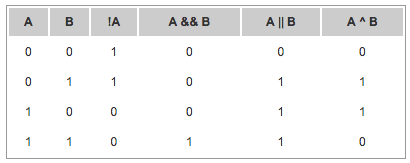
\includegraphics[width=.85\textwidth]{figuras/boolean.png}
		\caption{Topcoder}
	\end{figure}
\end{center}

\end{block}

\end{frame}

%- - - - - - - - - - - - - - - - - - - - - - - - - - - - - - - - - SLIDE -
\begin{frame}
\frametitle{Estruturas de Dados (continuação)}
\begin{block}{Bitmask}
A versão bit a bit destas operações funciona da mesma forma, mas ao invés de interpretar seus argumentos como verdadeiro ou falso, eles operam sobre cada bit dos argumentos. Logo, se A é 1010 e B é 1100, então:
\begin{itemize}
	\bitem A \& B = 1000
	\bitem A | B = 1110
	\bitem A \^\ B = 0110
	\bitem $\sim$A = 11110101 (o numero de 1's depende no número de bits do tipo de A).
\end{itemize}
\end{block}
\end{frame}

%- - - - - - - - - - - - - - - - - - - - - - - - - - - - - - - - - SLIDE -
\begin{frame}
\frametitle{Estruturas de Dados (continuação)}
\begin{block}{Bitmask}
\begin{itemize}
	\bitem Outros dois operadores que precisaremos são os \textit{shift operators} $a << b$ e $a >> b$. O primeiro faz um \textit{shift} de todos os bits em $a$ para a esquerda por $b$ posições. O segundo faz a mesma coisa mas o \textit{shift} é pra direita.
	\bitem Para valores não negativos (que são os que estamos interessados), os novos bits que aparecem com os \textit{shifts} são zeros.
	\bitem Podemos considerar \textit{shifts} de $b$ bits para a esquerda como uma multiplicação por $2^b$ e para a direira como divisão inteira por $2^b$.
	\bitem Um dos usos mais comuns de \textit{shifts} bit a bit são para acessar um bit em particular. Por exemplo, $1 << x$ é um número binário com o bit $x$ setado e os outros não setados(bits são quase sempre contados como sendo o menos significante o mais a direita, o qual tem índice 0).
\end{itemize}
\end{block}
\end{frame}

%- - - - - - - - - - - - - - - - - - - - - - - - - - - - - - - - - SLIDE -
\begin{frame}
\frametitle{Estruturas de Dados (continuação)}
\begin{block}{Bitmask}
\begin{itemize}
	\bitem Em geral, usamos um inteiro para representar um conjunto em um domínio de até 32 valores (ou 64, usando um inteiro de 64 bits), com um bit setado representando um valor que está presente no conjunto e um bit não setado representando um valor que não está presente no conjunto.
	\bitem Sabendo disso, as seguintes operações são bem intuitivas, onde ALL\_BITS é um número com 1's para todos os bits correspondendo aos elementos do domínio:
	\begin{itemize}
		\bitem União de conjuntos: A | B
		\bitem Intersecção de conjuntos: A \& B
		\bitem Subtração de conjuntos: A \& $\sim$B
		\bitem Negação de conjuntos: ALL\_BITS \^\ A
		\bitem Setar um bit: A |= 1 << bit
		\bitem Limpar um bit: A \&= $\sim$(1 << bit)
		\bitem Testar um bit: (A \& 1 << bit) != 0
	\end{itemize}
\end{itemize}
\end{block}
\end{frame}

%- - - - - - - - - - - - - - - - - - - - - - - - - - - - - - - - - SLIDE -
\begin{frame}
\frametitle{Estruturas de Dados (continuação)}
\begin{block}{Bitset}
\begin{itemize}
	\bitem Esta representação com inteiros entretanto é muito limitada, sendo esta limitação de apenas o maior inteiro representado pela linguagem, que normalmente é um inteiro de 64 bits.
	\bitem Para lidar com conjuntos maiores, existe uma implementação na STL que satisfaz esta necessidade com alguma perda de performance chamada \textit{bitset}.
\end{itemize}
\end{block}

\end{frame}

%- - - - - - - - - - - - - - - - - - - - - - - - - - - - - - - - - SLIDE -
\begin{frame}
\frametitle{Estruturas de Dados (continuação)}
\begin{block}{Bitset}
\begin{itemize}
	\bitem Operadores usados nas bitmasks também podem ser usados com bitsets:
	\begin{itemize}
		\bitem \&, |, \^\ , <<, >>, $\sim$
	\end{itemize}
	\bitem Além destes, vários outras funcionalidades são implementadas
\end{itemize}
\end{block}
\end{frame}

%- - - - - - - - - - - - - - - - - - - - - - - - - - - - - - - - - SLIDE -
\begin{frame}
\frametitle{Estruturas de Dados (continuação)}
\begin{block}{Bitset}
\begin{itemize}
	\bitem Acesso a bits pelo operador [ ]
	\bitem set() -- Seta os bits do bitset
	\bitem reset() -- Reseta os bits do bitset
	\bitem flip() -- Inverte os bits do bitset
	\bitem to\_ulong() -- Retorna o bitset convertido para um unsigned long
	\bitem to\_string() -- Retorna o bitset convertido para uma string
	\bitem count() -- Retorna o número de bits ativos
	\bitem size() -- Retorna o número de bits do bitset
	\bitem test(pos) -- Retorna se o bit na posição \textit{pos} está setado
\end{itemize}
\end{block}
\end{frame}
%- - - - - - - - - - - - - - - - - - - - - - - - - - - - - - - - - SLIDE -
\begin{frame}
\frametitle{Leituras Recomendadas}

\begin{block}{}
\begin{itemize}
\tiny
	\bitem \url{http://community.topcoder.com/tc?module=Static&d1=tutorials&d2=bitManipulation}
	\bitem \url{http://www.codechef.com/wiki/tutorial-bitwise-operations}
	\bitem \url{http://www.comp.nus.edu.sg/~stevenha/visualization/bitmask.html}
	\bitem \url{http://inf.ufg.br/~paulocosta/tap/material/bitmask.pdf}
\end{itemize}
\end{block}

\end{frame}

